\documentclass[tikz, border=14pt]{standalone}
\usepackage{tikz}
\usepackage{amsmath}
\usepackage{amssymb}
\usetikzlibrary{shapes.geometric, arrows.meta, positioning, fit, backgrounds, calc}

%% Color palette
\colorlet{Cenc}{blue!65!black}
\colorlet{Cinit}{orange!80!black}
\colorlet{Cdyn}{violet!75!black}
\colorlet{Cctrl}{red!65!black}
\colorlet{Cdec}{green!60!black}

\tikzset{
  %% Named block styles
  encbox/.style={draw=Cenc, fill=Cenc!8, rounded corners=4pt,
    text width=5.4cm, align=center, minimum height=1.1cm, thick, font=\small},
  initbox/.style={draw=Cinit, fill=Cinit!8, rounded corners=4pt,
    text width=5.4cm, align=center, minimum height=1.1cm, thick, font=\small},
  dynbox/.style={draw=Cdyn, fill=Cdyn!8, rounded corners=4pt,
    text width=5.6cm, align=center, minimum height=1.1cm, thick, font=\small},
  ctrlbox/.style={draw=Cctrl, fill=Cctrl!8, rounded corners=4pt,
    text width=5.6cm, align=center, minimum height=1.1cm, thick, font=\small},
  decbox/.style={draw=Cdec, fill=Cdec!8, rounded corners=4pt,
    text width=5.6cm, align=center, minimum height=1.1cm, thick, font=\small},
  iobox/.style={draw=black!40, fill=black!5, rounded corners=4pt,
    text width=5.4cm, align=center, minimum height=0.85cm, font=\small\itshape},
  %% Arrow styles
  arr/.style={-{Stealth[length=7pt, width=5pt]}, thick},
  darr/.style={-{Stealth[length=6pt, width=4pt]}, thick, dashed, black!40},
  %% Annotation label
  dim/.style={font=\tiny, text=black!50},
}

\begin{document}
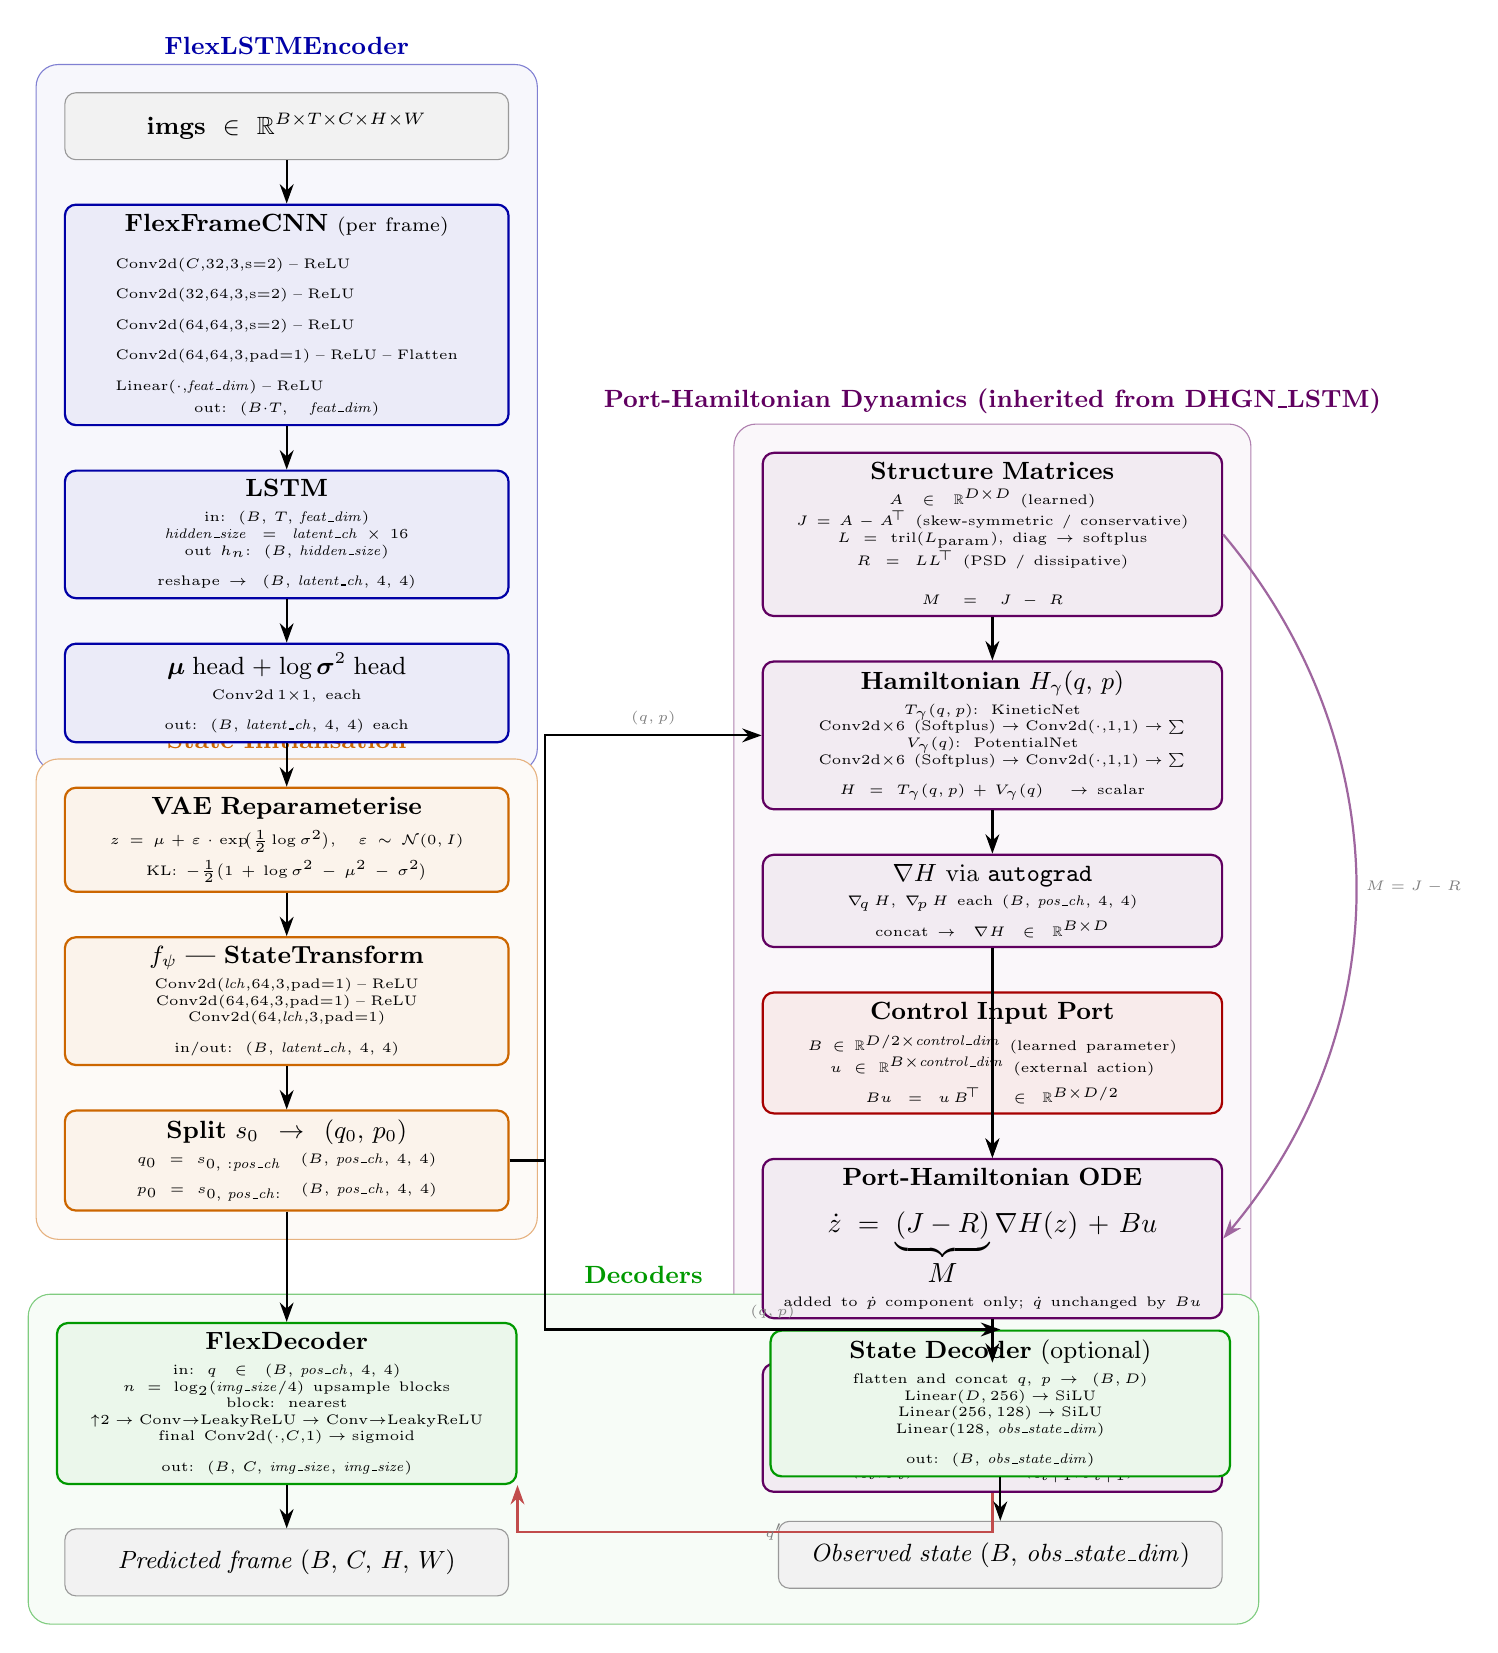
\begin{tikzpicture}[node distance=0.55cm and 3.2cm]

%%==========================================================================
%% LEFT COLUMN — Encoder + State Initialisation
%%==========================================================================

\node[iobox] (imgs)
  {$\mathbf{imgs}\in\mathbb{R}^{B\times T\times C\times H\times W}$};

\node[encbox, below=of imgs] (framecnn)
  {\textbf{FlexFrameCNN} \textnormal{\scriptsize(per frame)}\\[3pt]
   \begin{tabular}{l}
     \tiny Conv2d($C$,32,3,s=2)\;--\;ReLU\\
     \tiny Conv2d(32,64,3,s=2)\;--\;ReLU\\
     \tiny Conv2d(64,64,3,s=2)\;--\;ReLU\\
     \tiny Conv2d(64,64,3,pad=1)\;--\;ReLU\;--\;Flatten\\
     \tiny Linear($\cdot$,$\mathit{feat\_dim}$)\;--\;ReLU\\
   \end{tabular}\\
   \tiny out: $(B{\cdot}T,\;\mathit{feat\_dim})$};

\node[encbox, below=of framecnn] (lstm)
  {\textbf{LSTM}\\[3pt]
   \tiny in: $(B,\,T,\,\mathit{feat\_dim})$\\
   \tiny $\mathit{hidden\_size}=\mathit{latent\_ch}\times 16$\\
   \tiny out $h_n$: $(B,\,\mathit{hidden\_size})$\\
   \tiny reshape $\to(B,\,\mathit{latent\_ch},\,4,\,4)$};

\node[encbox, below=of lstm] (heads)
  {$\boldsymbol{\mu}$\;head\;+\;$\log\boldsymbol{\sigma}^2$\;head\\[3pt]
   \tiny Conv2d\,$1{\times}1$, each\\
   \tiny out: $(B,\,\mathit{latent\_ch},\,4,\,4)$ each};

\node[initbox, below=of heads] (reparam)
  {\textbf{VAE Reparameterise}\\[3pt]
   \tiny $z = \mu + \varepsilon\cdot\exp\!\bigl(\tfrac{1}{2}\log\sigma^2\bigr),\quad\varepsilon\sim\mathcal{N}(0,I)$\\
   \tiny KL: $-\tfrac{1}{2}\bigl(1+\log\sigma^2-\mu^2-\sigma^2\bigr)$};

\node[initbox, below=of reparam] (fpsi)
  {$f_\psi$ \textbf{— StateTransform}\\[3pt]
   \tiny Conv2d($\mathit{lch}$,64,3,pad=1)\;--\;ReLU\\
   \tiny Conv2d(64,64,3,pad=1)\;--\;ReLU\\
   \tiny Conv2d(64,$\mathit{lch}$,3,pad=1)\\
   \tiny in/out: $(B,\,\mathit{latent\_ch},\,4,\,4)$};

\node[initbox, below=of fpsi] (split)
  {\textbf{Split} $s_0\to(q_0,\,p_0)$\\[3pt]
   \tiny $q_0=s_{0,\;:\mathit{pos\_ch}}$\quad$(B,\,\mathit{pos\_ch},\,4,\,4)$\\
   \tiny $p_0=s_{0,\;\mathit{pos\_ch}:}$\quad$(B,\,\mathit{pos\_ch},\,4,\,4)$};

%%==========================================================================
%% RIGHT COLUMN — Dynamics
%%==========================================================================

\node[dynbox, right=of lstm] (structmat)
  {\textbf{Structure Matrices}\\[3pt]
   \tiny $A\in\mathbb{R}^{D\times D}$ \textnormal{(learned)}\\
   \tiny $J = A - A^{\!\top}$ \textnormal{(skew-symmetric / conservative)}\\
   \tiny $L = \mathrm{tril}(L_\mathrm{param})$, diag $\to$ softplus\\
   \tiny $R = LL^{\!\top}$ \textnormal{(PSD / dissipative)}\\[3pt]
   \tiny $M = J - R$};

\node[dynbox, below=of structmat] (hamnet)
  {\textbf{Hamiltonian} $H_\gamma(q,\,p)$\\[3pt]
   \tiny $T_\gamma(q,p)$: \textnormal{KineticNet}\\
   \tiny\quad Conv2d$\times$6 (Softplus)\;$\to$\;Conv2d($\cdot$,1,1)\;$\to$\;$\sum$\\
   \tiny $V_\gamma(q)$: \textnormal{PotentialNet}\\
   \tiny\quad Conv2d$\times$6 (Softplus)\;$\to$\;Conv2d($\cdot$,1,1)\;$\to$\;$\sum$\\
   \tiny $H = T_\gamma(q,p) + V_\gamma(q)\;\to$ scalar};

\node[dynbox, below=of hamnet] (gradH)
  {$\nabla H$ \textnormal{via} \texttt{autograd}\\[3pt]
   \tiny $\nabla_{\!q}\,H$, $\nabla_{\!p}\,H$ each $(B,\,\mathit{pos\_ch},\,4,\,4)$\\
   \tiny concat $\to \nabla H \in\mathbb{R}^{B\times D}$};

\node[ctrlbox, below=of gradH] (ctrl)
  {\textbf{Control Input Port}\\[3pt]
   \tiny $B\in\mathbb{R}^{D/2\times\mathit{control\_dim}}$ \textnormal{(learned parameter)}\\
   \tiny $u\in\mathbb{R}^{B\times\mathit{control\_dim}}$ \textnormal{(external action)}\\
   \tiny $Bu = u\,B^{\!\top}\;\in\mathbb{R}^{B\times D/2}$};

\node[dynbox, below=of ctrl] (ode)
  {\textbf{Port-Hamiltonian ODE}\\[5pt]
   \normalsize$\dot{z} = \underbrace{(J-R)}_{\displaystyle M}\nabla H(z) + Bu$\\[3pt]
   \tiny added to $\dot p$ component only; $\dot q$ unchanged by $Bu$};

\node[dynbox, below=of ode] (rk4)
  {\textbf{RK4 Integrator} \textnormal{(zero-order hold on $u$)}\\[3pt]
   \tiny 4 ODE evaluations per step (shared $M$)\\
   \tiny $(q_t,p_t)\;\xrightarrow{+\Delta t}\;(q_{t+1},p_{t+1})$};

%%==========================================================================
%% BOTTOM ROW — Decoders
%%==========================================================================

\node[decbox, below=1.4cm of split] (flexdec)
  {\textbf{FlexDecoder}\\[3pt]
   \tiny in: $q\in(B,\,\mathit{pos\_ch},\,4,\,4)$\\
   \tiny $n=\log_2(\mathit{img\_size}/4)$ upsample blocks\\
   \tiny block: nearest $\uparrow$2\;$\to$\;Conv$\to$LeakyReLU\;$\to$\;Conv$\to$LeakyReLU\\
   \tiny final Conv2d($\cdot$,$C$,1)\;$\to$\;sigmoid\\
   \tiny out: $(B,\,C,\,\mathit{img\_size},\,\mathit{img\_size})$};

\node[decbox, right=of flexdec] (statedec)
  {\textbf{State Decoder} \textnormal{(optional)}\\[3pt]
   \tiny flatten and concat $q$, $p$ $\to (B, D)$\\
   \tiny Linear$(D,256)$\;$\to$\;SiLU\\
   \tiny Linear$(256,128)$\;$\to$\;SiLU\\
   \tiny Linear$(128,\,\mathit{obs\_state\_dim})$\\
   \tiny out: $(B,\,\mathit{obs\_state\_dim})$};

\node[iobox, below=of flexdec]  (imgout)  {Predicted frame $(B,\,C,\,H,\,W)$};
\node[iobox, below=of statedec] (obsout)  {Observed state $(B,\,\mathit{obs\_state\_dim})$};

%%==========================================================================
%% ARROWS
%%==========================================================================

%% — Encoder pipeline
\draw[arr] (imgs)    -- (framecnn);
\draw[arr] (framecnn)-- (lstm);
\draw[arr] (lstm)    -- (heads);
\draw[arr] (heads)   -- (reparam);
\draw[arr] (reparam) -- (fpsi);
\draw[arr] (fpsi)    -- (split);

%% — split → FlexDecoder (direct)
\draw[arr] (split.south) -- (flexdec.north);

%% — split → State Decoder
\draw[arr] (split.east) -- ++(0.45,0) |-
  node[near end, above, dim] {$(q,p)$}
  (statedec.north);

%% — split → Hamiltonian (cross to right column)
\draw[arr] (split.east) -- ++(0.45,0) |-
  node[near end, above, dim] {$(q,p)$}
  (hamnet.west);

%% — Structure matrices pipeline
\draw[arr] (structmat) -- (hamnet);

%% — M from structmat to ODE (along right edge)
\draw[arr, Cdyn!60, bend left=40] (structmat.east) to
  node[right, dim, pos=0.5] {$M=J-R$} (ode.east);

%% — Dynamics pipeline
\draw[arr] (hamnet) -- (gradH);
\draw[arr] (gradH)  -- (ode);
\draw[arr] (ctrl)   -- (ode);
\draw[arr] (ode)    -- (rk4);

%% — RK4 output q′ → FlexDecoder (rollout path)
\draw[arr, Cctrl!70] (rk4.south) -- ++(0,-0.5) -|
  node[near start, right, dim] {$q'$}
  (flexdec.south east);

%% — Decoder outputs
\draw[arr] (flexdec) -- (imgout);
\draw[arr] (statedec)-- (obsout);

%%==========================================================================
%% BACKGROUND GROUPING BOXES
%%==========================================================================
\begin{scope}[on background layer]
  \node[draw=Cenc!50, fill=Cenc!3, rounded corners=8pt, inner sep=10pt,
    fit=(imgs)(framecnn)(lstm)(heads),
    label={[Cenc, font=\small\bfseries]above:FlexLSTMEncoder}] {};

  \node[draw=Cinit!50, fill=Cinit!3, rounded corners=8pt, inner sep=10pt,
    fit=(reparam)(fpsi)(split),
    label={[Cinit, font=\small\bfseries]above:State Initialisation}] {};

  \node[draw=Cdyn!50, fill=Cdyn!3, rounded corners=8pt, inner sep=10pt,
    fit=(structmat)(hamnet)(gradH)(ctrl)(ode)(rk4),
    label={[Cdyn, font=\small\bfseries]above:Port-Hamiltonian Dynamics  (inherited from DHGN\_LSTM)}] {};

  \node[draw=Cdec!50, fill=Cdec!3, rounded corners=8pt, inner sep=10pt,
    fit=(flexdec)(statedec)(imgout)(obsout),
    label={[Cdec, font=\small\bfseries]above:Decoders}] {};
\end{scope}

\end{tikzpicture}
\end{document}
